\section{What the native ANSYS benchmarks verify}\label{sec:nativebench}
The conduction check begins with a known radial temperature profile above a
22~$^\circ$C baseline. The inner and outer faces are held at 22~$^\circ$C.
For a homogeneous hollow cylinder the first radial diffusion mode has the form
$T(r,t)-22=\phi(r)\exp[-kt\lambda^2/(\rho c_p)]$, where $\phi$ vanishes at
both boundaries. After one decay time the temperature rise is $1/e$ of its
initial value everywhere. MAPDL advanced 256 substeps over 21.135~s on a sector
of 256 bricks with 585 nodes. The largest nodal error was 0.079~K against a
predeclared limit of 0.25~K. The root-mean-square error was 0.055~K.
\begin{figure}[H]\centering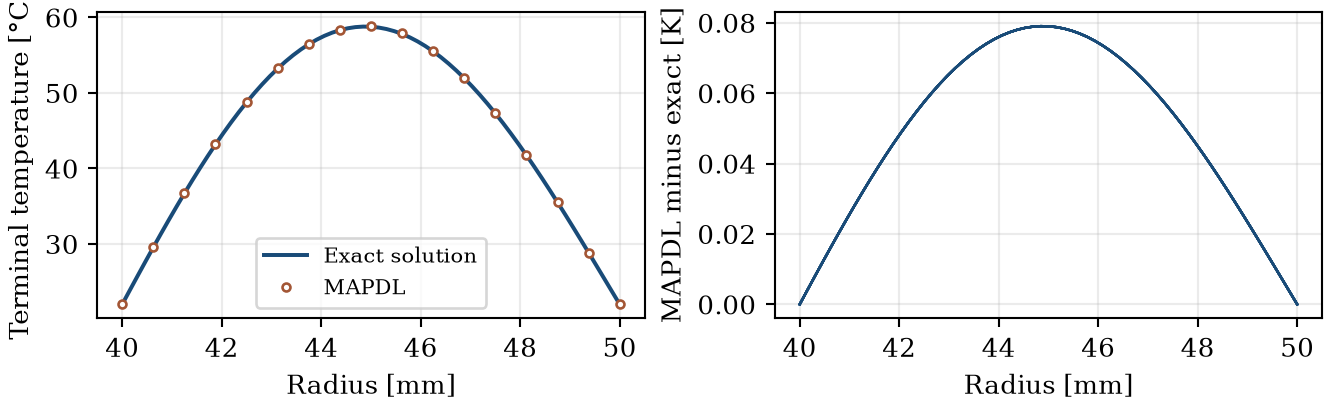
\includegraphics[width=.95\textwidth]{../analysis/native_annular_comparison.png}
\caption{At left, the native solution and analytical profile after one decay time.
At right, the signed error over all nine axial and angular node lines.}
\end{figure}
\paragraph{Receding char.} A second benchmark uses a 0.6~mm pure-char wall
with a prescribed logarithmic temperature profile and a corresponding heating
law. The code computes the face temperature, char mass flux and remaining
radius. Integration of the analytical recession speed gives an independent
reference time. A first implementation distorted connected elements while
moving nodes and also produced oscillating temperatures under a lagged
surface heat sink. The revised calculation rebuilds each brick after moving
all nodes and uses the local derivative of net incident flux to couple heating
and char consumption. Narrower transverse dimensions and a shared final time
interval control the aspect ratio as the remaining char becomes thin.
\begin{center}\begin{tabular}{rrrrr}\toprule
Radial cells & Steps & MAPDL [s] & Exact [s] & Error [\%]\\\midrule
8 & 41 & 8.1165 & 8.1297 & 0.162 \\
16 & 82 & 8.1231 & 8.1297 & 0.081 \\
\bottomrule\end{tabular}\end{center}
\paragraph{Motor field checks.} For each of the four geometries, MAPDL advanced
a frozen 30~s state through ten increments spanning 0.05~s. Across all four
cases the largest nodal difference from a separate brick assembly was 8.16$\times10^{-6}$~K.
These comparisons test heat storage and transport with the material state and
loads held fixed over that interval.
\paragraph{Separate pulse control.} In the final 320-row CF control, heating
ended at 7~s. The casing continued to warm during cooling and first exceeded
150~$^\circ$C between 29.4375 and 29.4687~s. At that point 4.718~mm of the original
4.7625~mm liner remained. All 5,295 accepted steps passed the balance checks.
The largest sampled native versus radial temperature difference was 0.0151~K.
The benchmarks on this page test conduction, moving geometry or pulse cooling.
The ignition-to-exhaustion times in the opening table still come from the two
independent radial simulations.
\clearpage
